\documentclass{beamer}

\mode<presentation>
{
  \usetheme{Luebeck} % Berlin,
  \usecolortheme{seahorse}
  \useoutertheme{infolines}
  %\usecolortheme[RGB={125,173,51}]{structure}
  % or ...
  %\setbeamercovered{transparent}
  % or whatever (possibly just delete it)
}

\usepackage[spanish]{babel}
\usepackage[utf8]{inputenc}
\usepackage{times}
\usepackage{multicol}
\usepackage{verbatim} 
\usepackage{fancyvrb}
\usepackage{graphicx}
\graphicspath{{images/}}
\usepackage{listings}
\usepackage{tikz}
\usetikzlibrary{arrows}
\usetikzlibrary{shapes}
\tikzstyle{block}=[draw opacity=0.7,line width=1.4cm]
\usepackage{hyperref}
\usepackage{xcolor}
\usepackage[breakable,listings,skins,hooks]{tcolorbox}
\hypersetup{
  colorlinks,
  allcolors=.,
  urlcolor=blue,
}

\usefonttheme[onlymath]{serif}

%\lstdefinelanguage{Marlowe}{%
  language     = Haskell,
  morekeywords = {Close, Pay, Assert, If, When, Let},
}
\lstdefinelanguage{Isabelle}{%
  language     = ML,
  morekeywords = {theory, imports, begin, end},
}

\definecolor{codegreen}{rgb}{0,0.6,0}
\definecolor{codegray}{rgb}{0.5,0.5,0.5}
\definecolor{codepurple}{rgb}{0.58,0,0.82}
\definecolor{backcolour}{rgb}{0.95,0.95,0.92}

\lstdefinestyle{Haskell-cardano}{
    backgroundcolor=\color{backcolour},   
    commentstyle=\color{codegreen},
    keywordstyle=\color{magenta},
    numberstyle=\tiny\color{codegray},
    stringstyle=\color{codepurple},
    basicstyle=\ttfamily\footnotesize,
    breakatwhitespace=false,         
    language=Haskell,
    breaklines=true,                 
    captionpos=b,                    
    keepspaces=true,                 
    numbers=none,                    
    numbersep=5pt,                  
    showspaces=false,                
    showstringspaces=false,
    showtabs=false,                  
    tabsize=2
}

\definecolor{isarblue}{HTML}{006699}
\definecolor{isargreen}{HTML}{009966}
\lstdefinelanguage{isabelle}{%
    keywords=[1]{type_synonym,datatype,fun,abbreviation,definition,proof,lemma,theorem, theory,corollary},
    keywordstyle=[1]\bfseries\color{isarblue},
    keywords=[2]{where,assumes,shows,and, imports, begin, end},
    keywordstyle=[2]\bfseries\color{isargreen},
    keywords=[3]{if,then,else,case,of,SOME,let,in,O},
    keywordstyle=[3]\color{isarblue},
}
\lstdefinestyle{Isabelle}{%
  language=isabelle,
  escapeinside={&}{&},
  columns=fixed,
  extendedchars,
  frame=single,
  basewidth={0.5em,0.45em},
  basicstyle=\ttfamily,
  mathescape,
}


\title[Verificación de smart contracts en Marlowe]% (optional, use only with long paper titles)
{Verificación de smart contracts en Marlowe para la blockchain Cardano}

\author[Julián Ferres] % (optional, use only with lots of authors)
{~Julián Ferres}
% - Give the names in the same order as the appear in the paper.
% - Use the \inst{?} command only if the authors have different
%   affiliation.
\institute[FIUBA] % (optional, but mostly needed)
{
  %\inst{1}
  Facultad de Ingeniería\\Universidad de Buenos Aires.
}
\date{\today}

% Acá se puede insertar el logo de la UBA
\pgfdeclareimage[height=0.6cm]{fiuba}{images/FIUBA_Logo.png}
\logo{\pgfuseimage{fiuba}}


% Tamaño de fuente en la primer página
\setbeamerfont{author}{size=\small}
\setbeamerfont{institute}{size=\scriptsize}
\setbeamerfont{date}{size=\scriptsize}

% Delete this, if you do not want the table of contents to pop up at
% the beginning of each subsection:
%\AtBeginSubsection[]
\AtBeginSubsection[]
{
  \begin{frame}{Índice de contenidos}
  \footnotesize
    %\begin{multicols}{2} 
    \tableofcontents[currentsection, currentsubsection]
    %\end{multicols}
  \end{frame}
}


\begin{document}
\pgfdeclarelayer{background}
\pgfsetlayers{background,main}

\begin{frame}
	\titlepage
\end{frame}


\begin{frame} 
	\footnotesize
	\frametitle{Índice de Contenidos}
	%\begin{multicols}{2} 
	\tableofcontents
	%\end{multicols}
\end{frame}

%# Esquema de temas para la presentación
%
%- Introducción
%    - Similar a lo contado en el primer capítulo del documento. Una breve descripción de que son, por que son importantes y las opciones de IOHK para:
%        - Blockchains
%        - Criptomonedas
%        - Smart contracts
%
%    - Un poco de introducción a ACTUS, mencionar porque es importante y útil dicho estandar (mencionando que Cardano planea implementar todos los contratos en el fúturo)
%        - Describir un poco el módelo que se utiliza (Scheduling, estado, inicialización de variables de estado, POFs y STFs) y mostrar algún fragmento de la tabla.
%
%    - Introducción a pruebas:
%        - Por qué es importante verificar contratos
%        - Algunas variantes y porque se utilizó Isabelle en Particular
%        - Un poco de descripción breve de Isabelle
%
%- Mostrar la escritura de contratos
%    - En esta sección me enfocaría más en describir lo necesario para escribir un contrato en Cardano, y quizas agregue algún snippet corto de alguna parte de los contratos que implementé. Esto es porque realmente es requerimiento entender el módelo del generador para empezar a ver como programar un nuevo contrato.
%
%
%- Mostrar y describir algunas de las pruebas:
%    - Va a ser necesario al menos una mención al modelo de Marlowe y las funciones más importantes implementadas en Isabelle, sino no se va a saber la utilidad de las funciones en las que estamos probando propiedades.
%    - Depende de las pruebas que decidamos mostrar, quizás mencionar un poco la motivación y técnicas de prueba que fui usando. 
%
%
%- Conclusión y cierre, hacer un breve comentario de los temas abordados y posibles fuentes de desarrollo que se desprenden de la tesis.

\section{Introducción}

\subsection{Blockchains, Criptomonedas y Smart contracts}

\begin{frame}{Cadenas de bloques o \textit{Blockchains}}
Las cadenas de bloques, conocidas en inglés como blockchains, son estructuras de datos en las cuales la información se divide en conjuntos (bloques) que cuentan con información adicional relativa a bloques previos de la cadena.
\smallskip

\pause

Con esta organización relativa, y con ayuda de técnicas criptográficas, la información de un bloque solo puede ser alterada modificando todos los bloques anteriores.
\smallskip

\pause

Esta propiedad facilita su aplicación en un entorno distribuido, de manera tal que la cadena de bloques puede modelar una base de datos pública no relacional, que contenga un registro histórico irrefutable de información.
\smallskip

\pause

En la práctica esta técnica ha permitido la implementación de un registro contable o ledger distribuido que soporta y garantiza la seguridad de transacciones y dinero digital. 

\end{frame}


\begin{frame}

\begin{figure}
    \centering
    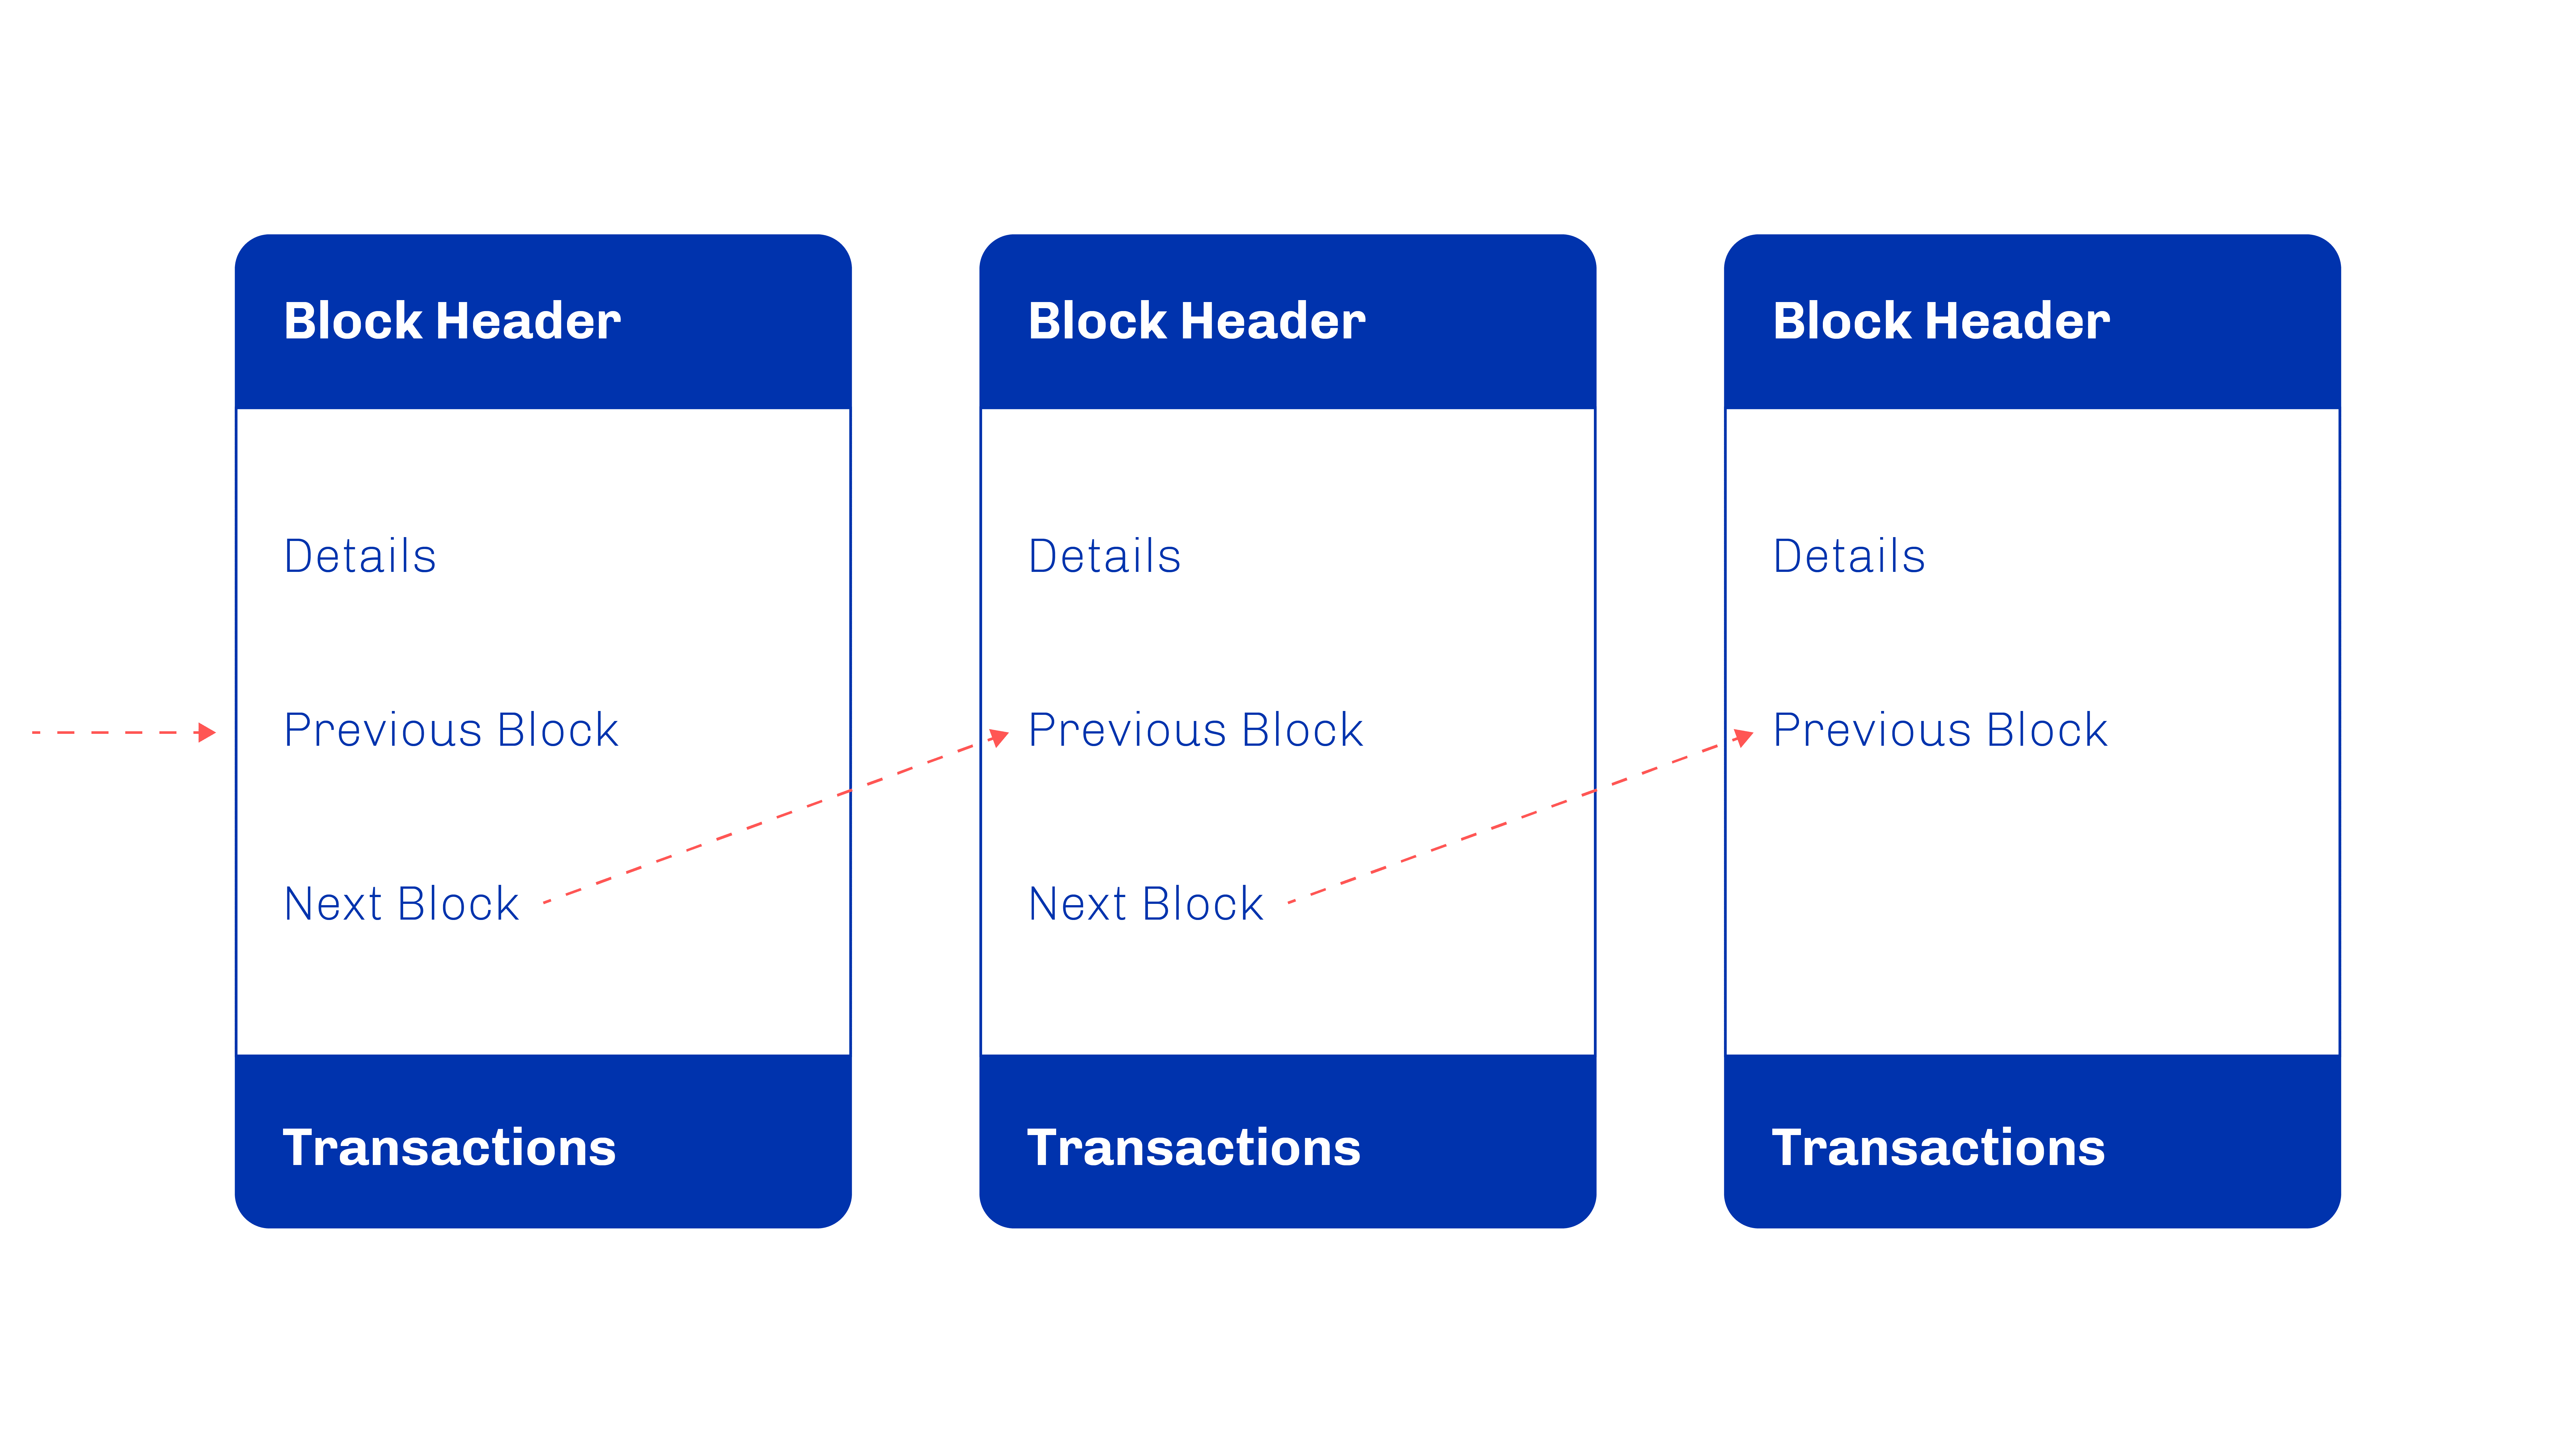
\includegraphics[width=0.9\textwidth]{Bloques.png}
    \caption[Representación simplificada de los datos en un bloque de la cadena.]{Representación simplificada de los datos en un bloque de la cadena. Extraída de~\cite{plutus-smart-contracts}.}\label{fig:Bloques}
\end{figure}


\end{frame}

\begin{frame}{Criptomonedas}
Las criptomonedas son activos digitales que se almacenan en el ledger y están diseñadas para servir como medio de intercambio de bienes o servicios. 
\smallskip

\pause

Los ledgers de blockchain son utilizados como tecnología subyacente para la creación de criptomonedas en un entorno descentralizado. 
\smallskip

\pause

Los protocolos de blockchain utilizan técnicas criptográficas rigurosas para permitir la creación de criptomonedas, asegurar y verificar la propiedad de las mismas y los registros de movimiento de fondos. 
\smallskip

\pause

El precio de la criptomoneda no está controlado por un gobierno o una institución financiera centralizada. Se define por su valor, la correlación con las cifras del mundo real y está impulsado por la oferta y la demanda del mercado. 

\end{frame}

\begin{frame}{\textit{Smart contracts}}
    Un contrato inteligente o \textit{smart contract} es un \underline{acuerdo digital automatizado}.
    \smallskip

\pause

    Los mismos están escritos en código, rastrean, verifican y ejecutan las transacciones de un contrato entre varias partes.
    \smallskip

\pause

Las transacciones del contrato se ejecutan automáticamente mediante el código del smart contract cuando se cumplen las condiciones predeterminadas. Esencialmente, un contrato inteligente es un programa cuyas entradas y salidas son acciones en una cadena de bloques.
\smallskip

\pause

Los smart contracts son auto-ejecutables y no requieren las acciones o la presencia de terceros. El código del contrato inteligente se almacena y distribuye en la \textit{blockchain}, lo que lo hace transparente e irreversible.

\end{frame}

\subsection{Cardano}

\begin{frame}
Cardano es una plataforma blockchain descentralizada de tercera generación, cuya criptomoneda es llamada \textit{ada}. 

\pause

\begin{itemize}
    \item \textbf{La primera generación} de blockchains (con Bitcoin como gran representante) ofrece ledgers descentralizados para la transferencia segura de criptomonedas. \pause Sin embargo, tales \textit{blockchains} no proporcionaron un entorno funcional para la liquidación de acuerdos complejos y el desarrollo de aplicaciones descentralizadas (dApps). 
    \pause

    \item \textbf{La segunda generación} (cuyo ejemplo más conocido es Ethereum) proporcionó soluciones mejoradas para redactar y ejecutar contratos inteligentes, desarrollar aplicaciones y crear diferentes tipos de tokens. \pause Sin embargo, la segunda generación de cadenas de bloques a menudo enfrenta problemas en términos de escalabilidad.
\end{itemize}
\end{frame}

\begin{frame}{Cardano como \textit{blockchain} de 3ra generación}

Cardano se concibe como la cadena de bloques de tercera generación.

La misma combina las propiedades de las generaciones anteriores y ofrece las siguientes propiedades:
\pause

\begin{itemize}
    \item \textbf{Seguridad}
        \pause
    \item \textbf{Escalabilidad}: Rendimiento de transacciones, escala de datos, ancho de banda de la red.
        \pause
    \item \textbf{Funcionalidad}: Además del procesamiento de transacciones, la cadena de bloques debe proporcionar todos los medios para la liquidación de acuerdos comerciales. 
        \pause
    \item \textbf{Desarrollo e Intregración}: Es importante asegurarse que la blockchain esté en constante desarrollo en términos de sostenibilidad y sea interoperable con otras blockchains e instituciones financieras.
\end{itemize} 

\end{frame}


\begin{frame}{Ada como criptomoneda de Cardano}
Cada ledger de blockchain tiene su criptomoneda subyacente o moneda nativa. Ada es la moneda
nativa o principal en Cardano. Esto significa que ada es la principal unidad de pago en Cardano.

\pause
\medskip

Cardano también admite la creación de \textbf{tokens nativos}: activos digitales que se crean para fines
específicos. 

\medskip
\pause

Por lo tanto los usuarios, desarrolladores y empresas pueden usar la cadena de bloques de Cardano para crear tokens que representen una huella de valor.

\pause
\medskip

Un token puede ser \textbf{fungible} (intercambiable) o \textbf{no fungible} (único) y actuar como unidad de pago, recompensa, activo
comercial o contenedor de información.

\end{frame}


\subsection{ACTUS}

\begin{frame}{Contratos Financieros}
Los contratos financieros son acuerdos legales entre dos (o más) partes sobre el futuro intercambio de dinero. Dichos acuerdos legales se definen sin ambigüedades por medio de un conjunto de términos y lógica contractual.

\pause
\vfill

Como resultado, los mismos pueden describirse matemáticamente y representarse mediante algoritmos.

\end{frame}

\begin{frame}
Los beneficios de representar contratos financieros de esta forma son múltiples:

\begin{itemize}
    \pause

    \item Tradicionalmente, el procesamiento de transacciones ha sido un campo en el que se pueden lograr mejoras de eficiencia mediante la automatización de contratos.

    \pause

    \item El análisis financiero se basa en la disponibilidad de representaciones computables de estos acuerdos, donde a menudo se utilizan aproximaciones analíticas. \pause Recientemente, el auge de las blockchain, de contabilidad distribuida y los diversos casos de uso de los contratos inteligentes han abierto nuevas posibilidades para los contratos financieros digitales.
\end{itemize}

\end{frame}

\begin{frame}
    En general, el intercambio de flujos de efectivo entre partes sigue ciertos patrones. \pause

    Un patrón típico es un contrato de préstamo de tipo \textit{bullet}: \pause

    \medskip

    \begin{quote}
        ``Se entrega un monto de dinero inicial, a cambio de pagos de intereses cíclicos y la devolución del dinero inicial en el vencimiento del contrato.''
    \end{quote}
    \pause
    \medskip

    Si bien los pagos son fijos, existen muchas variantes que determinan cómo se programan y/o pagan los pagos de intereses cíclicos:
    \begin{itemize}
        \pause
        \item Los pagos de intereses pueden ser mensuales, anuales, mediante períodos arbitrarios. 
        \pause
        \item Las tasas pueden ser de fijas o variables.
        \pause
        \item Pueden usarse diferentes métodos de cálculo de fracciones anuales o que no haya ningún interés.
    \end{itemize}



\end{frame}


\subsection{Verificación formal}

\begin{frame}{Concepto general, herramientas y metodologías}
Los asistentes de pruebas formales son herramientas de software diseñadas para ayudar a sus usuarios a realizar pruebas, especialmente en cálculo lógico.

\medskip

Por lo general, los llamamos asistentes de demostración o demostradores interactivos de teoremas.

\medskip
\pause

La principal fortaleza de los asistentes de prueba es que ayudan a desarrollar pruebas altamente confiables e inequívocas de enunciados matemáticos, usando lógica precisa. Se pueden usar para probar resultados arbitrariamente avanzados, y no solo ejemplos simples.

\end{frame}

\begin{frame}{Algunos asistentes de pruebas}

Hay una gran cantidad de asistentes de prueba en desarrollo o uso alrededor del mundo. A
continuación presentamos una lista de los principales, clasificados por sus fundamentos lógicos:
\medskip
\pause

\begin{itemize}
    \item \textbf{Teoría de conjuntos}: Isabelle/ZF, Metamath, Mizar
    \item \textbf{Teoría simple de tipos}: HOL4, HOL Light, Isabelle/HOL
    \item \textbf{Teoría dependiente de tipos}: Agda, Coq, Lean, Matita, PVS
    \item \textbf{Lógica de primer orden, de tipo Lisp}: ACL2
\end{itemize}
\end{frame}

\section{Escribiendo contratos ACTUS en Cardano}

\subsection{Contratos en Cardano}

\begin{frame}

\end{frame}

\section{Verificando propiedades en contratos en Marlowe}

\subsection{El modelo de Marlowe}

\subsection{Pruebas sencillas sobre contratos específicos}

\subsection{Warnings en Auction}

\section{Conclusión}

\subsection{Resumen}

\subsection{Posibles temas de desarrollo futuro}


\section{Bibliografía}
\begin{frame}[allowframebreaks]{Bibliografía}
    \bibliographystyle{apalike}
    \bibliography{bibliografia.bib}
\end{frame}

\end{document}
